% Chapter Template

\chapter{Experimento: Buscando el Efecto Espejo en una tarea Perceptual} % Main chapter title

\label{Cap_Exp} % Change X to a consecutive number; for referencing this chapter elsewhere, use \ref{ChapterX}

%----------------------------------------------------------------------------------------
%	SECTION 1
%----------------------------------------------------------------------------------------
\section{Planteamiento general}

%Se propone buscar evidencia del Efecto Espejo en una tarea fuera de Memoria de reconocimiento


%Se propone una tarea perceptual ya que carece de una fase de preparacion
El interés principal del trabajo aquí expuesto es evaluar la posibilidad de que el Efecto Espejo y los patrones de respuesta reportados en estudios de memoria de reconocimiento como parte del mismo, sean producto de la aplicación del modelo de detección de señales en la comparación del desempeño de los participantes en dos condiciones de dificultad (i.e. dos niveles de d') y no así de una discrepancia a nivel de procesos superiores de atención, procesamiento y memoria que determine la distribución de dichos grupos de estímulos en el eje de la evidencia. Para ello se diseñó una tarea de detección meramente perceptual, donde las condiciones de dificultad fueron construidas con base en su discriminabilidad perceptual.\\ 

%Se trabaja con ilusiones opticas, dado que la literatura en ellas permite anticiparnos a la d' y proponer dos niveles de dificultad.
Las ilusiones ópticas 

\subsection{Objetivo}

%Buscar evidencia del efecto espejo en una tarea de detección que no implique el reconocimiento de estimulos ya conocidos.
Poner a prueba la existencia de los patrones de respuesta identificados como parte del Efecto Espejo en una tarea de detección perceptual con dos niveles de dificultad, (i.e. una tarea de detección que no pertenezca a la familia de tareas de reconocimiento y, principalmente, que carezca de una etapa previa a la fase experimental donde los participantes tuvieran ocasión de manipular los estímulos y dar un trato distinto a cada nivel de dificultad).\\

\section{Construcción de los Experimentos}

%La tarea de detección princiál consiste en comparar el tamaño de dos círculos en pantalla, donde uno de ellos o ambos podía estar construido como una Figura de Ebbinghaus (dependiendo del Experimento)
Para poner a prueba la extensión del Efecto Espejo a fenómenos más allá de la memoria de reconocimiento, se diseñó una tarea de detección perceptual donde el objetivo de los participantes era señalar aquellos ensayos en que dos círculos a comparar fueran del mismo tamaño, indicando si éste era el caso ensayo a ensayo presionando una de dos posibles teclas. Se construyeron dos variaciones de esta tarea donde, para controlar la dificultad de la tarea, solo uno de estos circulos, o ambos, fueron construidos como parte de una figura de Ebbinghaus (variaciones a las cuales nos referiremos como Experimento 1 y Experimento 2, respectivamente).\\ 

%Descripcion de la Ilusión de Ebbinghaus, la composición de la figura y cómo se explica.
La ilusión de Ebbinghaus (a.k.a. Círculos de Titchner) refiere a un fallo en la estimación del tamaño de un círculo cuando este aparece rodeado por un halo de círculos uniformes de mayor o menor tamaño (Ver Figura~\ref{fig:Ebbinghaus}). La ilusión suele explicarse como producto de la interferencia producida por la estructura de los estímulos sobre el sistema cognoscitivo-perceptual que estima el tamaño de los estímulos en relación a cómo contrastan éstos con su entorno ($REFERENCIA$). De tal forma que la ilusión de Ebbinghaus comprende dos posibles efectos sobre la estimación del tamaño del círculo central: la subestimación y la sobrestimación; la primera de ellas, refiere a cuando el círculo central se encuentra rodeado por un halo de círculos de mayor tamaño que inducen la subestimación de su tamaño y, la segunda, implica el caso contrario en que los círculos externos son más pequeños que el círculo central y llevan al espectador a percibir a este último como más grande de lo que en realidad es.\\

\begin{figure}[th]
\centering

\includegraphics[width=0.55\textwidth]{Figures/Ebbinghaus} 
\decoRule
\caption[Ilusión de Ebbinghaus ejemplar]{Ilustración de la Ilusión de Ebbinghaus. Los círculos centrales de ambas figuras son del mismo tamaño. Sin embargo, el círculo central de la figura izquierda tiende a ser percibido como más pequeño (efecto de subestimación) y el círculo derecho suele ser percibido como más grande (efecto de sobrestimación), como producto del contraste que guardan con los círculos circundantes.}
\label{fig:Ebbinghaus}
\end{figure}

%Factores o variables que han demostrado influir en la intensidad de la ilusión.
La intensidad de la ilusión de Ebbinghaus (i.e. la desviación inducida en la estimación del tamaño del círculo central en relación a su tamaño real) está relacionada con tres variables: 

\begin{itemize}
\item El tamaño de los círculos externos.
\item La distancia entre el círculo central y el halo de círculos externos.
\item El número de círculos externos.
\end{itemize}

%Descripción del procedimiento empleado por Massaro y Anderson para probar la influencia del numero de circulos externos y el tamaño de los mismos en la Ilusión de Ebbinghaus.
La Figura~\ref{fig:Ebb_Var} muestra los resultados de uno de los experimentos conducidos por \parencite{Massaro1971} para evaluar el efecto de las variables involucradas en las figuras de Ebbinghaus en la magnitud de la ilusión. Para dicho experimento, se trabajó con figuras de Ebbinghaus construidas con un diseño factorial de 2x3x5: dos posibles tamaños del círculo central (13 y 17 mm); tres niveles de 'número de círculos externos' (dos, cuatro y seis); cinco niveles del tamaño de los círculos externos que diferían del círculo central en -8, -4, 0, 4 y 8 mm; la distancia entre el círculo central y los externos se mantuvo constante para todas las figuras. Por cada figura de Ebbinghaus presentada, los participantes tenían que elegir de entre un set de círculos de comparación aquel cuyo diámetro se aproximara más al círculo central de la figura de Ebbinghaus (i.e. 27 círculos aislados que variaban en tamaño dentro de un rango  de 8.5 a 21.5 mm en saltos de 0.5 mm).\\

%Descripción de los resultados encontrados por Massaro y Anderson en el mismo estudio.
La figura~\ref{fig:Ebb_Var} reportada por \parencite{Massaro1971} muestra el diámetro promedio del círculo de comparración elegido como 'igual' al círculo central de las figuras de Ebbinghaus (los autores promediaron entre ambos valores de círculo central), a lo largo de los distintos niveles de número de círculos externo, por cada tamaño implementado de círculos externos. El efecto de ambas variables se muestra de manera clara: mientras más círculos externos se presentan en la figura de Ebbinghaus, mayor es la intensidad de la ilusión (i.e. aumenta la distancia entre el valor real del tamaño del círculo central y la estimación de los participantes), como se puede observar en la tendencia que siguen las pendientes; mientras mayor sea la diferencia entre el tamaño del círculo central y los círculos externos, la ilusión aparece con mayor intensidad, como se puede observar por la distancia vertical que separa cada una de las líneas trazadas. En la figura se puede distinguir claramente entre el efecto de sobreestimación (inducido por las figuras cuyos círculos externos eran más pequeños que el círculo central), y subestimación, (donde las figuras tienen círculos externos más grandes que el círculo central). \\

\begin{figure}[th]
\centering
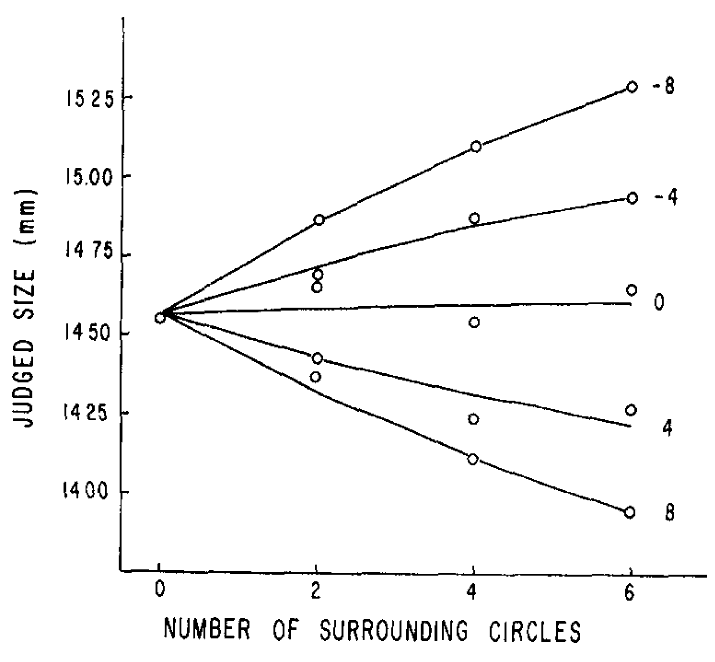
\includegraphics[width=0.55\textwidth]{Figures/Ebb_Variables} 
\decoRule
\caption[Efecto del Numero y Tamaño de los círculos externos en la Ilusión de Ebbinghaus]{Se muestra el efecto que tienen el número de círculos externos incluídos en la ilusión de Ebbinghaus (eje x) sobre los fallos en la estimación del tamaño del círculo central (eje Y); se muestran con líneas diferentes los resultados obtenidos por ilusiones de Ebbinghaus donde los círculos externos diferían en tamaño del círculo central con los valores especificados. La figura fue extraída de la investigación conducida por \parencite{Massaro1971}; Figura 2}
\label{fig:Ebb_Var}
\end{figure}

%Las condiciones de dificultad estarán determinadas por el número de círculos externos
De acuerdo con los hallazgos reportados por \parencite{Massaro1971}, se decidió trabajar con el número de círculos externos como factor determinante para la construcción de dos niveles de d'. La tarea de detección propuesta contaría con una condición fácil (i.e. D' mayor) donde las figuras de Ebbinghaus estuvieran compuestas por pocos círculos externos (2 o 3 círculos) y una condición difícil (i.e. D' menor) con más círculos externos (7 u 8 círculos externos).\\ 

\subsection{Diseño de los Estímulos}

%En el experimento se trabajó con figuras de Ebbinghaus que promovieran efecto de subestimación Y sobrestimación del tamaño. 
Las figuras de Ebbinghaus diseñadas para los experimentos propuestos incluían los dos tipos de ilusiones. Se construyeron figuras que favorecían la sobrestimación y la subestimación utilizando dos tamaños fijos para los círculos externos (5 cm y 1 cm, respectivamente). El tamaño de los círculos externos en las figuras de subestimación (5 cm) se eligió de manera tal que estos fueran más grandes que todos los tamaños de círculo central empleados (entre 1 y 3 cm, en saltos de 0.5 cm). El tamaño utilizado para las figuras de sobreestimación (1cm) se eligió procurando que los circulos externos fueran más pequeños que la mayoría de los círculos centrales a utilizar. Arbitrariamente, dada la configuración de la pantalla a utilizar para correr los experimentos, se decidió sacrificar la relación con el círculo central más pequeño (también de 1cm de diámetro), cancelando -en teoría- la existencia de cualquier efecto sobre la estimación de su tamaño. La razón por la que se incluyeron tanto figuras con efecto de sobrestimación como subestimación fue la de prevenir la habituación y la fatiga de los participantes durante la tarea, dotándole de cierto dinamismo con una mayor variabilidad en los estímulos presentados. Los tamaños de círculos externos propuestos se mantuvieron constantes a lo largo de los distintos niveles de 'número de círculos externos' en cada condición. Dado que el objetivo principal de la esta investigación es comparar el desempeño de los participantes entre las condiciones de dificultad propuestas, el posible efecto diferencial que pudieran tener los tamaños de círculos externos elegidos en su interacción con los tamaños de círculo central probados no se controló en el diseño de las figuras dado que esta relación permaneció constante entre las condiciones a comparar.\\

%No se controló la distancia entre el círculo central y los círculos externos.
En ninguno de los experimentos realizados se controló la distancia entre el círculo central y el halo de círculos externos. Al construir las figuras de Ebbinghaus el halo de círculos externos se formó de acuerdo al número de círculos externos, comenzando con las figuras de la condición difícil que contenían entre 7 y 8 círculos externos. Una vez habiendo distribuido los 7 u 8 círculos externos de manera equidistante entre sí en torno al círculo central, se usaron estas mismas figuras como base para la construcción de estímulos de la condición fácil con 2 o 3 círculos externos, borrando los círculos sobrantes y respetando la ubicación de los restantes respecto del círculo central; para las figuras con 2 círculos externos, se procuró que estos estuvieran enfrentados en puntos opuestos del círculo central y para las figuras con tres círculos centrales se procuró que estos estuvieran localizados de manera tal que formasen un ángulo de $CIENTO VEINTE GRADOS$ entre sí. El tamaño impuso una restricción importante en la formación de estos halos de 7 u 8 círculos externos, por lo que su localización permaneció constante a lo largo de los distintos tamaños de círculo central, modificando en consecuencia la distancia entre estos. Es en este sentido que se habla de una falta de control en la distancia entre los círculos centrales y el halo de círculos externos. Sin embargo, apelando nuevamente a que dichas distancias permanecen constantes entre condiciones de dificultad, no se consideró una fuente de ruido importante para analizar lo que se propuso en la tarea: diferencias en el desempeño dependientes del número de círculos externos.\\

A continuación, se desarrolla con detalle la construcción de los estímulos (Señales y ruido) utilizados en cada uno de los dos experimentos realizados. Las especificaciones respecto al procedimiento, las tareas y los controles realizados en los experimentos se explican a profundidad, más adelante.\\

\begin{itemize}
\item Experimento 1 : Circulo de referencia aislado vs Figura de Ebbinghaus.

%Los ensayos de la tarea de detección están compuestos por un círculo aislado constante del lado izquierdo, cuyo tamaño debe ser comparado con el círculo central de una figura de Ebbinghaus en el lado derecho de la pantalla.
En el Experimento 1 sólo se mostraba una figura de Ebbinghaus por ensayo, siempre en la mitad derecha de la pantalla, cuyo círculo central los participantes tenían que comparar con un círculo de referencia de 2 cm de diámetro, con localización fija en la mitad izquierda de la pantalla, para determinar si su tamaño era el mismo (señal) o no (ruido). Los círculos a comparar aparecían a la misma altura de la pantalla. El círculo de referencia y el círculo central de las figuras de Ebbinghaus aparecían 14 cm a la izquierda y 10 cm a la derecha del centro de la pantalla, respetivamente.\\

%Desarrollo del diseño factorial de 5x2x2 utilizado para construir los estímulos del Experimento 1: 5 circulos centrales x 2 tipos de ilusion x 2 niveles de 'numero de circulos externos'
Las figuras de Ebbinghaus utilizadas en el Experimento 1 se diseñaron de acuerdo a un diseño factorial de 5x2x2, (Ver Figura~\ref{fig:Exp_1}). Se utilizaron cinco diferentes tamaños de círculo central, partiendo del tamaño del círculo de referencia (2 cm; la combinación con la señal) y alejándose de este en saltos de 0.5 cm en ambas direcciones (i.e. Círculos más pequeños que la referencia, de 1 y 1.5 cm, y círculos más grandes que la referencia, de 2.5 y 3 cm de diámetro). Por cada uno de estos cinco tamaños de círculo central, se construyeron dos tipos de figuras de Ebbinghaus dependientes del tamaño de los círculos externos: grande (efecto de subestimación) y pequeño (efecto de sobrestimación). Por último, por cada una de estas 10 combinaciones, se hicieron dos figuras diferentes de acuerdo a los niveles de 'número de círculos externos' propuestos por condición (2 y 3 círculos en la condición fácil; 7 y 8 círculos en la condición difícil). Esto nos deja con un subtotal de 20 figuras diferentes por condición y un total de 40 en todo el experimento.\\
 
%Los estímulos con ruido se presentaron 10 veces durante el experimento. Los estímulos con señal se presentaron con 40 repeticiones. La discrepancia en el número de repeticiones entre ambos tipos de estímulo se hizo para igualar la  
El set de figuras de Ebbinghaus construido contiene una mayor cantidad de estímulos con ruido (32 figuras con ruido; 16 por condición) que con señal (8 figuras con la señal; 4 por condición). Para procurar que los participantes se encontraran con la misma cantidad de ensayos con señal que con ensayo con ruido, se incrementó el número de repeticiones con que las figuras con señal aparecieron en el experimento. Cada una de las 32 figuras de Ebbinghaus con ruido se presentó en diez ocasiones diferentes durante el experimento, mientras que las ocho figuras con señal tuvieron 40 repeticiones por cada una. De esta forma, el experimento terminó compuesto por 320 ensayos con ruido y 320 ensayos con señal, 160 ensayos por cada condición de dificultad para ambos tipos de estímulo. La inclusión homogénea de ensayos con ruido y señal se realizó con el fin de que la discrepancia en la aparición de un caso sobre otro no proviera información que sesgara la respuesta de los participantes hacia la emisión de juicios negativos ('No, no son iguales').\\

\begin{figure}[th]
\centering
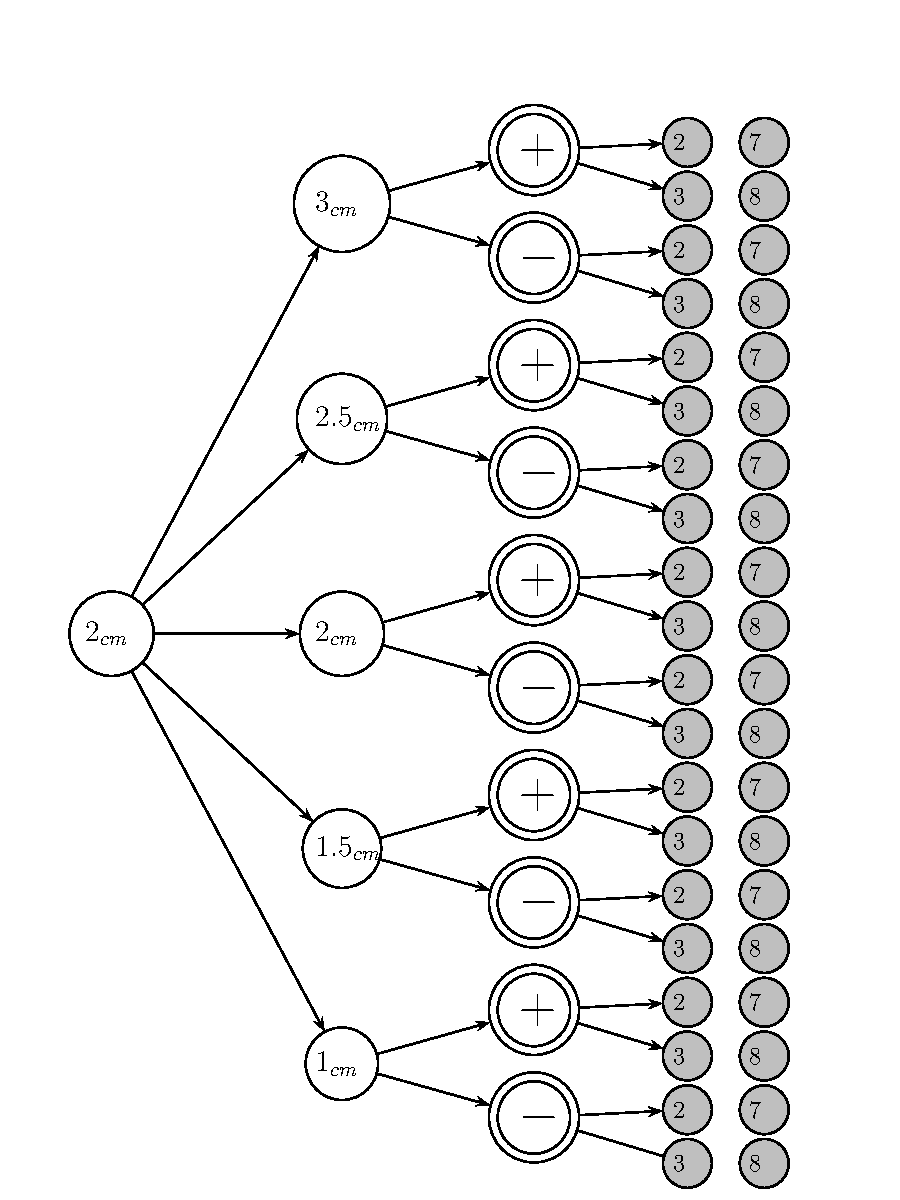
\includegraphics[width=0.99\textwidth]{Figures/Estimulos_Experimento1} 
\decoRule
\caption[Diseño de Estimulos en el Experimento 1]{Diseño factorial (5x2x2) utilizado para construir los estímulos utilizados durante la tarea de detección en el Experimento 1. En cada ensayo los participantes tenían que comparar el tamaño de un círculo de referencia constante con el círculo central de una figura de Ebbinghaus, que podía aparecer en cinco posibles tamaños, con círculos externos que inducen efectos de sobrestimación o subestimación (indicado en el esquema con  y signos positivos y negativos, respectivamente) y con dos niveles de 'número de círculos externo' por condición (2 y 3 círculos externos en la condición fácil o 7 y 8 en la condición difícil). Por cada condición de dificultad, se tienen 16 estímulos con ruido, (10 repeticiones por cada uno, en cinco colores diferentes) y 4 que contienen la señal (repetidos 40 veces cada una, en cinco colores diferentes), dejándonos con 320 ensayos por condición y un total de 640 ensayos en el experimento.}
\label{fig:Exp_1}
\end{figure}

%Las repeticiones de cada figura aparecieron en cinco colores diferentes para prever la fatiga.
Procurando evitar la fatiga en los participantes, cada uno de los estímulos diseñados apareció en cinco colores diferentes (Guinda, Anaranjado, Verde, Azul y Púrpura) en cantidades iguales (Dos estímulos de cada color dentro de las 10 repeticiones de estímulos con ruido y 8 estímulos de cada color dentro de las 40 repeticiones de estímulos con señal). Para todos los casos, el círculo central se mostró en un tono más claro que los círculos externos. Estas diferencias en el tono y color de las figuras han demostrado no tener un efecto en la intensidad de la ilusión $REFERENCIA$ y fueron incluidas con la única intención de tener una mayor variabilidad en los estímulos presentados y que los participantes no se harten ni se aburran de la tarea, ambos estados que podrían mermar la atención con que responden a la misma. 

\item Experimento 2 : Figura de Ebbinghaus (Sobrestimación) vs Figura de Ebbinghaus (Subestimación).

%En la tarea de detección, los participantes tenían que comparar el círculo central de dos figuras de Ebbinghaus que aparecían simultáneamente en la pantalla: una con círculos externos grandes (Efecto de subestimación)  y una con círculos externos pequeños (Efecto de sobrestimación).
En el Experimento 2 los participantes tenían que comparar el tamaño del círculo central de dos figuras de Ebbinghaus que aparecían simultáneamente en pantalla. Al igual que en el Experimento 1, las respuestas se reportaban presionando una de dos posibles teclas para señalar si los círculos a comparar tenían el mismo tamaño (la señal) o no (el ruido). Las parejas construidas contenían ambos tipos de ilusiones: una figura con efecto de subestimación (con círculos externos grandes; 6 cm de diámetro) y una figura con efecto de sobrestimación (con círculos externos pequeños; 1 cm de diámetro). Los círculos centrales aparecían en pantalla a la misma altura, a -15 y 11 cm respecto del centro de la pantalla.\\


%Se formaron cinco parejas con la Señal (cinco pares iguales de tamaño de círculo central) y cinco parejas con el ruido (cuatro cuyos círculos centrales diferían en 0.5 cm y una que difería en 1 cm).
La Figura~\ref{fig:Exp_2} ilustra el diseño de las figuras de Ebbinghaus utilizadas en el Experimento 2. A diferencia del Experimento 1, donde uno de los círculos a comparar permanecía constante, en el Experimento 2 se varió el diámetro de los dos círculos a comparar dentro de un rango de cinco valores, de 1 a 3 cm en saltos de 0.5 cm, construyendo así cinco tipos posibles de Parejas-señal. Por su parte, las Parejas-ruido se formaron arbitrariamente, empatando círculos centrales cuyo diámetro difiriese en 0.5 cm (i.e 1 vs 1.5 cm; 1.5 vs 2 cm; 2 vs 2.5 cm y 2.5 vs 3 cm), con una quinta pareja donde la diferencia se extendía hasta 1 cm, entre los valores menos extremos (1.5 cm vs 2.5 cm). Para cada una de estas 10 parejas, se crearon cuatro nuevas versiones para cada condición, de acuerdo con las posibles combinaciones de los niveles de 'número de círculos centrales' (2 círculos externos a ambos lados, 3 círculos externosa ambos lados, 2 en izquierdo y 3 en derecho y 3 en izquierdo y 2 en derecho, para la condición fácil; 7 círculos externos a ambos lados, 8 círculos externos ambos lados, 7 círculos del lado izquierdo y 8 en el derecho y 8 círculos en el lado izquierdo y 7 en el derecho). En total, el Experimento 2 estuvo compuesto por 80 parejas diferentes de figuras de Ebbinghaus cuyos círculos centrales debían compararse; 40 por condición; 20 por cada tipo de estímulo en cada condición.\\

\begin{figure}[th]
\centering
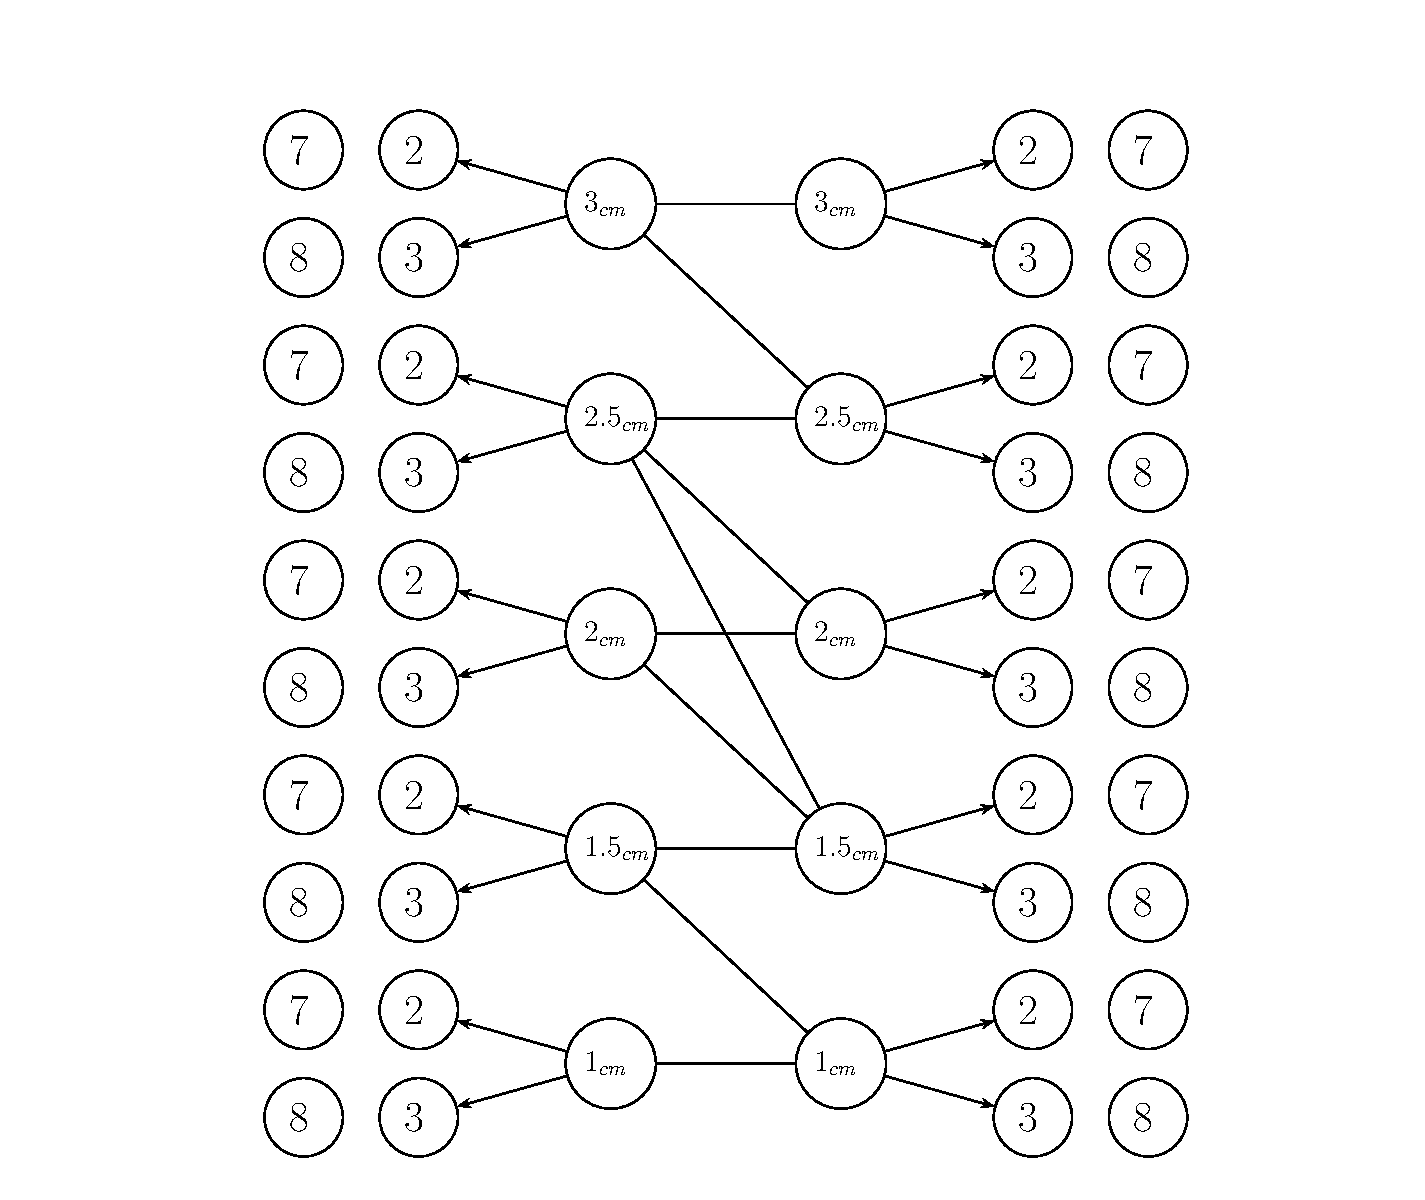
\includegraphics[width=1.2\textwidth]{Figures/Estimulos_Experimento2} 
\decoRule
\caption[Diseño de Estimulos en el Experimento 2]{Diseño de las parejas  de figuras de Ebbinghaus a comparar en el Experimento 2. Se manejaron cinco tamaños distintos de círculo central, que se mostraron en parejas iguales (cinco señales) y cinco parejas desiguales (cuatro cuyos círculos centrales diferían en 0.5 cm y, una con una diferencia de 1 cm). En cada pareja siempre había una figura de Ebbinghaus que inducía la subestimación del tamaño central y una que promovía la subestimación, contrabalanceando el orden en que aparecían en pantalla (relativo a la posición izquierda o derecha). Por cada pareja de círculos centrales, se contemplaron cuatro combinaciones posibles entre los dos niveles de círculos externos contenidos por cada condición (i.e. a vs a, b vs b, a vs b, b vs a; donde a y b son sustituíbles por 2 y 3 círculos externos en la condición fácil o 7 y 8, en la condición difícil.)}
\label{fig:Exp_2}
\end{figure}
\end{itemize}

%Cada pareja diseñada se repitió 8 veces; en 4 colores diferentes y contrabalanceando la ubicación de cada tipo de ilusión. En total, el Experimento 2 estuvo compuesto por 640 ensayos.
Cada una de las 80 parejas diseñadas para el Experimento 2 se presentó 8 veces, en cuatro colores diferentes (púrpura, anaranjado, azul y verde) para prevenir la fatiga de los participantes, contrabalanceando además la ubicación de las ilusiones de sobrestimación y subestimación a la derecha o izquierda de la pantalla. En otras palabras, por cada pareja construida de figuras a comparar se incluyeron ocho ensayos en el experimento: con un par de cada uno de los cuatro colores propuestos, dentro de los cuales se variaba la localización de las ilusiones a la derecha o izquierda, con un caso de cada combinación posible (i.e. Sobrestimación - Subestimación vs Subestimación - Sobrestimación). De tal forma que el Experimento 2 estuvo compuesto por un total de 640 ensayos; 320 por cada condición y 160 por cada tipo de estímulo por condición.\\ 

\subsection{Materiales}

%Programacion de la tarea
La tarea fue programada y ejecutada en PsychoPy v.12, un paquete de libre acceso programado en lenguaje Python que facilita la generación de tareas experimentales en psicología y neurociencias.  

%Detalles sobre la Mac y el espacio utilizado para correr el experimento.
El experimento se corrió en una computadora de escritorio Mac, con una pantalla de $medidas$, en un cubículo interno dentro del laboratorio 25 del Edificio D de la Facultad de Psicología de la UNAM.

\subsection{Participantes}

%Total de participantes y distribucion entre experimentos.
Un total de cuarenta y un estudiantes de la Facultad de Psicología participaron en los experimentos planteados: veinte en el Experimento 1 y veintiuno en el Experimento 2. Los experimentos se llevaron a cabo de manera simultánea. Los participantes fueron asignados a los experimentos alternadamente, procurando terminar con una cantidad similar de participantes en cada uno.\\

%Procedencia y generalidades sobre los participantes.
Todos los participantes fueron estudiantes de los primeros cuatro semestres de la licenciatura en Psicología de la Facultad de Psicología de la Universidad Nacional Autónoma de México, cuyas edades variaban entre los 18 y los 21 años. Su participación fue incentivada con el ofrecimiento de un boleto para la rifa de una tarjeta de regalo con valor de $TRESCIENTOS PESOS$ pesos para la plataforma de su preferencia entre iTunes, Netflix y Amazon. Se realizaron dos rifas independientes, una por cada experimento. Sin embargo, pese a que se informó a los participantes de la existencia de dos experimentos diferentes con su respectiva rifa, nunca se les proporcionó información respecto a cuál habían sido asignados.\\ 

%Consentimiento informado.
Para participar en el experimento se solicitó a cada participante que firmara una carta de consentimiento individual donde se les informaba la duración estimada de la tarea (40 minutos para cualquiera de los experimentos), se confirmaba su participación en una de las rifas y se les advertía que el procedimiento podría resultar fatigoso y que, aunque su participación era voluntaria y podían dimitir en cualquier momento, su permanencia en el mismo hasta el final era crucial para poder utilizar sus datos. De manera adicional, todos los participantes proporcionaron número(s) de teléfono y correo electrónico como medio de contacto.\\

\section{Procedimiento}

%Los experimentos propuestos difieren en el tipo de estímulos a presentar. Sin embargo, la tarea principal y el resto de los detalles del procedimiento permanecen iguales para ambos casos. 
La diferencia primordial entre los Experimentos 1 y 2 tiene que ver con el tipo de estímulos presentados a los participantes: en un caso se compara el círculo central de una figura de Ebbinghaus contra un círculo de referencia fijo (Experimento 1) y en el otro, se muestran simultáneamente dos figuras de Ebbinghaus cuyos círculos centrales deben compararse. La tarea es la misma (comparar el diámetro de dos círculos específicos que se muestran en la pantalla), de la misma forma que el resto del procedimiento a seguir y los detalles con que este fue programado.\\

%La tarea de detección constaba de dos fases: 1) Una tarea de detección binaria (¿Son o no del mismo tamaño?) y 2) Una tarea con escala de confianza (¿Qué tan seguro estás de tu respuesta?)
Los experimentos incorporaron dos procedimientos diferentes para evaluar la tarea de detección propuesta: una pregunta de respuesta binaria 'Sí/No' y una escala de confianza sobre esta primer respuesta.\\

Después de haber firmado la carta de consentimiento informado, se instalaba a los participantes en el espacio asignado para la realización del experimento. En el monitor de la computador designada se mostraba una pantalla inicial que daba la bienvenida a los participantes al Laboratorio 25 de la Facultad de Psicología de la Universidad Nacional Autónoma de México. En cuanto el participante oprimía la barra espaciadora comenzaban a desplegarse las instrucciones para responder al experimento ($REFERENCIA A APENDICES$), que incluían un ejemplo de cómo se verían los estímulos a comparar de acuerdo con el experimento realizado. Las instrucciones finalizaban con una pantalla en blanco con la leyenda 'Presiona la barra espaciadora para comenzar el experimento', que daba oportunidad a los participantes de comenzar el experimento en cuanto estuvieran listos.\\

La estructura de cada ensayo fue la siguiente:\\

\begin{itemize}
\item Fase 1: Tarea de respuesta binaria 'Sí/No'

En esta primera fase, se mostraba a los participantes los círculos a comparar para que indicaran, presionando una de dos posibles teclas, si sus diámetros eran o no del mismo tamaño. Si los círculos eran percibidos como iguales, los participantes debían presionar la tecla 'S'; en caso contrario, 'N'.

En cada ensayo se mostró a los participantes uno de los estímulos a comparar acompañado por un par de leyendas en la parte superior e inferior de la pantalla, respectivamente. Estas leyendas fueron colocadas a manera de recordatorio para los participantes: en la parte superior de la pantalla se les recordaba la pregunta de detección a responder (i.e. ¿Los círculos centrales son del mismo tamaño?) y en la parte inferior, las teclas que debían presionar para emitir su respuesta (i.e. 'S = Sí, N = No'). Como ejemplo de cómo se veían los ensayos experimentales en los Experimentos 1 y 2, ver las Figuras $FIGURAS DE EJEMPLO$, respectivamente.\\

Los estímulos se mostraban en pantalla sólo por 1.5 segundos para preveer la habituación de los participantes a la ilusión, con independencia de si se hubiera emitido una respuesta antes de finalizado el intervalo. Si el participante respondía antes de 1.5 s, los estímulos se quedaban en pantalla hasta terminar dicho periodo, tras el cual se avanzaba inmediatamente a la siguiente fase del ensayo. Si el participante no había registrado su respuesta aún después de la desaparición del estímulo, las leyendas-recordatorios permanecían en pantalla hasta que esta fuese emitida.\\

\item Fase 2: Escala de Confianza

%En una segunda fase, los participantes tuvieron que oprimir una tecla del 1 al 3 para indicar qué tan seguros estaban de la respuesta recién emitida.
Una vez registrada la respuesta de los participantes a la tarea 'Sí/No', comenzaba la Fase 2 del ensayo. En esta ocasión, los participantes tenían que presionar una tecla del 1 al 3 que reflejara qué tan seguros se sentían de la respuesta recién dada en la fase anterior. Para esto, se desplegaba en pantalla una tabla que recordaba a los participantes las opciones de respuesta y su significado (i.e. '1, Poco seguro; 2, Más o menos seguro; 3, Muy seguro') debajo de la pregunta guía '¿Qué tan seguro estás de tu respuesta?'. \\

El puntaje asignado por el participante (1,2,3) para valuar su seguridad en la respuesta dada a la tarea binaria 'Sí/No' fue convertido y registrado por el programa como parte de una escala más grande, con valores del 1 al 6, que distingue entre la seguridad que se tiene en que el estímulo a evaluar es un ensayo con ruido y la seguridad en que se trata de una señal.

\end{itemize}

%Entre cada ensayo, se presentó una pantalla intermedia que solicitaba a los participantes presionar la barra espaciadora para indicar que estaban listos para responder al siguiente ensayo.
Una vez registrado el puntaje asignado por el participante a la escala de confianza, se mostraba una pantalla intermedia entre ensayos que indicaba a los participantes que presionaran la barra espaciadora cuando estuvieran listos para atender y responder al siguiente ensayo con una nueva pareja de estímulos. Estas pantallas entre ensayos fueron incluidas para garantizar que los participantes pudieran atender y evaluar los círculos a comparar durante el periodo de exposición de los mismos.\\

%Se registraron tiempos de respuesta por cada respuesta registrada (Respuesta en la tarea Sí/No; Respuesta en la escala de confianza) y  la duración del experimento completo.
Se registraron los tiempos de respuesta de los participantes a las diferentes fases del experimento. Por cada ensayo, se registró el tiempo de respuesta de los participantes a la tarea binaria tras la aparición de los estímulos a comparar en pantalla y el tiempo de respuesta a la escala de confianza. También se registró el tiempo total de duración del experimento, comenzando desde que los participantes presionaban la barra espaciadora para ver las instrucciones hasta que terminaran de responder al último de los 640 ensayos, cuando recibían la retroalimentación global del número de aciertos y errores.\\

%Controles
Se controló que la distancia que separase los estímulos presentados se encontrara dentro de un ángulo de $X grados$ del campo visual de los participantes, así como que estos realizaran la tarea en una distancia de 1 m respecto del monitor.



\subsection{Registro de respuestas}

El experimento fue programado de manera tal que por cada participante se obtuviera un documento en formato csv (i.e. comma separated value) que contuviera información, ensayo a ensayo, sobre la respuesta dada por 
